\documentclass[a4paper,12pt,french]{article}
\usepackage[margin=2cm]{geometry}
\usepackage[thinfonts,latinmath]{uglix2}
\nouveaustyle

%
%\aut{intitulé}
%
\newcounter{autNum}
\setcounter{autNum}{0}
%
\newcommand{\aut}[1]
{
	\addtocounter{autNum}{1}
	{\titlefont\color{bleufonce@color}\Large Automatisme\ \theautNum\ \normalsize{#1}}\smallskip	
}


\begin{document}
\titre{Raisonnements}{Automatismes 1}{\premiere}

\setlength{\columnsep}{50pt}
\setlength{\columnseprule}{1pt}

Pour chaque automatisme, répondre à la question posée en explicitant le raisonnement.\\

\begin{multicols}{2}

	
	\aut{ Vrai ou faux ?}\\
	Si $\quad x\leqslant2$, \quad alors $\quad x^2\leqslant4$.
	\vspace{1.5cm}
	
	\aut{}\\
	On construit une succession de triangles :\\
	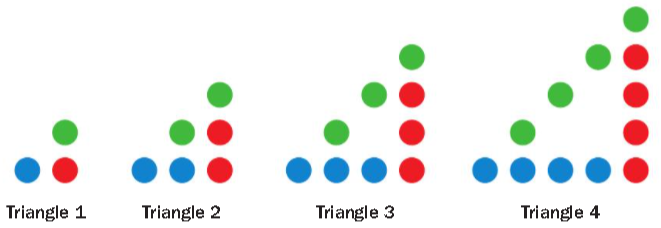
\includegraphics[width=8cm]{triangles}\\
	
	Combien de balles sont nécessaires pour construire le triangle 5 ?\\
	
	Conjecturer le nombre de balles nécessaires pour construire le triangle $n$.
	\vspace{1.5cm}
	
	\aut{ Vrai ou faux ?}\\
	Si $\quad x\leqslant-1$, \quad alors $\quad x^2\geqslant1$.
	\vspace{1.5cm}
	
	\aut{}\\
	Je parie sur un nombre.\\
	On lance deux dés à six faces et on calcule la somme des deux dés.\\
	Si mon nombre est égal à la somme obtenue, je gagne.\\
	Sur quel nombre dois-je parier pour avoir le plus de chances de gagner ?
	
	\vspace{1.5cm}
	
	\aut{}\\
		\begin{minipage}{4.5cm}
		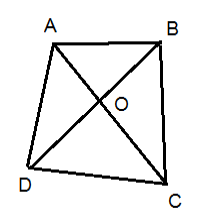
\includegraphics[width=3.5cm]{quadrilatere}
	\end{minipage}
	\begin{minipage}{5cm}
		$AO=$ 25 cm\\
		$BO=$ 25 cm\\
		$CO=$ 25 cm\\
		$DO=$ 25 cm
	\end{minipage}
	Quelle est la nature du quadrilatère $ABCD$ de centre $O$ ?\\
	\vspace{0.5cm}
	
	\aut{ Vrai ou faux ?}
	$$\dfrac{3}{2}+\dfrac{12}{8}=\dfrac{15}{10}$$
	\vspace{0.5cm}
	
	\aut{ Vrai ou faux ?}\\
	Pour tous nombres réels $a, b, c$ et $d$ non nuls :
	$$\dfrac{a}{b}+\dfrac{c}{d}=\dfrac{a+c}{b+d}$$
	\vspace{0.5cm}
	
	\aut{ Vrai ou faux ?}\\
	Si un nombre est multiple de 3, alors son carré est multiple de 3.\\
	\vspace{0.5cm}
	
	\aut{ Vrai ou faux ?}\\
	Un quadrilatère qui a ses diagonales de même longueur est un rectangle.\\
	\vspace{0.5cm}
	
	\aut{ Vrai ou faux ?}\\
	Si un nombre n'est pas multiple de 3, alors son carré n'est pas multiple de 3. 
\end{multicols}

\end{document}
